\documentclass[brazil,times]{abnt}
\usepackage[pdfborder={0 0 0}]{hyperref}
\usepackage[T1]{fontenc}
\usepackage[utf8]{inputenc}
\usepackage{url}
\usepackage{graphicx}
\usepackage{amssymb}
\makeatletter
\usepackage{babel}
\makeatother

\begin{document}

\autor{Pedro Paulo Vezzá Campos \\ Daniel Moraes Huguenin \\ Antonio Rui Castro
Junior}

\titulo{Guerra Das Universidades: \\Manual do Desenvolvedor}

\comentario{Manual do desenvolvedor do projeto desenvolvido pela Equipe Knuth
apresentado para avaliação na disciplina MAC0242, do curso de Bacharelado em
Ciência da Computação, turma 45, da Universidade de São Paulo, ministrada pelo
professor Roberto Hirata Junior.}

\instituicao{Departamento de Ciência da Computação \par Instituto de Matemática
e Estatística \par Universidade de São Paulo}

\local{São Paulo - SP, Brasil}

\data{\today}

\capa

\folhaderosto

\tableofcontents

\chapter{Introdução}
Este relatório apresenta os desenvolvimentos e resultados dos trabalhos da
Equipe Knuth - Pedro Paulo Vezzá Campos, Daniel Moraes Huguenin e Antonio Rui
Castro Junior que resultaram na produção do jogo \textbf{Guerra das
Universidades}.

Instruções de compilação e execução estão disponíveis em
\cite{compilacao-execucao}. Instruções de como jogar e a especificação do
projeto estão disponíveis em \cite{manual-usuario}. O blog de desenvolvimento
encontra-se em \url{http://guerradasuniversidades.wordpress.com}. O repositório
de código está em \url{http://code.google.com/p/guerradasuniversidades}.

\chapter{Cronologia}

\section{Fase 0 - Especificação}
Para o projeto da disciplina MAC0242 - Laboratório de Programação II foi
sugerido pelo professor Hirata a implementação de um jogo com temática
universitária aos moldes de jogos famosos, tais como \emph{Civilization} ou
\emph{SimCity}. Para isso, deveriam ser utilizandos os conceitos de Programação
Orientada a Objetos (POO) vistos em aula, linguagem Java e um \emph{framework}
de desenvolvimento de jogos, inicialmente com a sugestão de utilização do PlayN
\cite{playn}.

\subsection{Decisões Tomadas}
Na fase 0 o grupo definiu através de \emph{mockups} e descrição textual o que
viria a ser posteriormente o Guerra Das Universidades. O jogo possui uma
temática semelhante a \emph{Age of Empires}, consistindo de um
ambiente de \emph{singleplayer} 2D com oponentes implementados como
Inteligências Artificiais (IA). O objetivo do jogador, que assume o papel de
reitor de uma universidade, é construir estruturas essenciais ao campus, recrutar
alunos e professores para atacar universidades inimigas enquanto se defende de
ataques de terceiros. Ganha a universidade que permanecer funcionando por mais
tempo.

Ainda, foi criado o blog de desenvolvimento onde os alunos podem apresentar seus
progressos e dificuldades no decorrer do desenvolvimento. O blog da Equipe Knuth
encontra-se em: \url{http://guerradasuniversidades.wordpress.com}. Por fim, os
manuais de desenvolvedor e usuário tiveram seus primeiros esboços produzidos. 

\subsection{Dificuldades Enfrentadas}
Conscientes do curto período de tempo que haveria para o desenvolvimento
completo do projeto a equipe decidiu por não tornar muito complexa a
especificação, transformando funcionalidades supérfluas tais como recursos
visuais mais complexos em opcionais a serem implementados caso haja
tempo suficiente para isso.

Em contrapartida, houve um comprometimento mútuo de \textbf{preservar ao máximo a
qualidade do código produzido}, o que trouxe posteriormente um aumento de
legibilidade, robustez e manutenibilidade do código.


\section{Fase 1 - Protótipo}
Na fase 1 foi proposto que os alunos codificassem um protótipo do jogo para
provar que o jogo é viável do ponto de vista de dificuldade de implementação e
jogabilidade.

\subsection{Decisões Tomadas}
O grupo decidiu apostar no uso do PlayN como framework para o desenvolvimento do
jogo por sugestão do professor e pela proposta ambiciosa dos desenvolvedores do
arcabouço de prover uma ferramenta que torne o desenvolvimento de jogos
agnóstico à plataforma a ser utilizada seja ela Java, HTML5, Flash ou Android.

Uma vez decidido isso, procedeu-se com a codificação quase total da interface
gráfica do jogo sem nenhum tipo de modelo lógico associado. Com isso, os alunos
tomaram maior familiaridade com as ferramentas utilizadas no processo e
adiantaram uma parte importante do desenvolvimento do projeto.

O protótipo gerado pode ser acessado em:
\url{http://pedrovc-playn-test.appspot.com}

\subsection{Dificuldades Enfrentadas}
A grande dificuldade enfrentada neste momento foi dominar o PlayN. O framework é
bastante recente e possui uma documentação \textbf{extremamente} escassa. A
comunidade de desenvolvedores está ainda se formando tornando fraca a oferta de
material de estudo como fóruns, tutoriais ou manuais. O
aprendizado concentrou-se nos exemplos fornecidos juntamente com o PlayN e
bastante experimentação.

Exemplos de problemas com o PlayN (E sua biblioteca auxiliar a tripleplay): A
pobreza de recursos como caixas de diálogo e disposição de elementos
graficamente na tela, problemas com a translação e atualização de layers com
botões clicáveis (Enfrentados na implementação do scroll de itens que podem ser
comprados).

Ainda, outra dificuldade foi coordenar o trabalho remoto dos integrantes devido
aos diversos conflitos de horário, entre estágios e matérias extras. Nos
reunimos poucas vezes (mas foram bem produtivas). Neste momento, o uso de um
repositório de código compartilhado foi crucial para permitir o progresso do
trabalho.


\section{Fase 2 - Continuação}
Devido a questões de cronograma esta fase foi suprimida da agenda de entregas a
ser respeitada pelas equipes.


\section{Fase 3 - Implementação do Modelo Lógico}
Nesta fase foi pedido que as equipes tenham implementado completamente seus
jogos.

\subsection{Decisões Tomadas}
Uma vez que as especificações foram melhor delineadas na fase 1, procedeu-se com
a implementação do modelo lógico de maneira isolada da interface gráfica. Para
isso, utilizou-se de uma interface em modo texto que simula as ações permitidas
pelo jogo.

Paralelamente, foram produzidos os testes unitários do modelo lógico utilizando
a biblioteca JUnit para garantir seu bom funcionamento. Para a parte gráfica,
os testes foram realizados visualmente e de maneira manual.

Em seguida foi realizada a junção da interface com o modelo. Neste momento foram
necessários pequenos ajustes na interface para adequar-se ao funcionamento do
modelo, além disso foram aperfeiçoadas as classes controle do jogo, configurando
um projeto MVC \cite{reenskaug-mvc}.

\subsection{Dificuldades Enfrentadas}
A implementação do modelo em si não trouxe grandes dificuldades exceto os
cuidados para manter o código dentro dos princípios da orientação a objetos. Foi
necessário o uso de algumas design patterns como \textbf{Observador-Observado},
\textbf{Fachada} e \textbf{MVC} para atingir este objetivo. Isto está detalhado
posteriormente na seção \ref{documentacao-codigo}.

Outra dificuldade foi o fato do GWT não disponibilizar o uso das classes
Observer e Observable do Java ao ser feito o deploy para o Google AppEngine.
Isso foi resolvido com o uso de uma implementação livre destas classes sob a
GPL.

\section{Fase 4 - Documentação}
Para a fase final do projeto foi requisitado que os alunos entregassem seus
projetos finalizados e documentados para avaliação.

\subsection{Decisões Tomadas}
Nesta fase a equipe decidiu documentar o código utilizando a sintaxe Javadoc o
que permitiu a geração automatizada de documentação acessível via navegador web.
O resultado encontra-se no diretório \texttt{Documentacao} do arquivo compactado
junto com os fontes do projeto, manuais, etc.

Ainda, foram feitos ajustes finos na interface que haviam sido deixados
incompletos em fases anteriores.

Por fim, foram completos os manuais de usuário, desenvolvedor e
compilação/execução.


\subsection{Dificuldades Encontradas}
A dificuldade enfrentada neste momento foi enfrentar o trabalho de documentar um
projeto que totaliza aproximadamente 3000 linhas de código entre modelo e
interface.


\chapter{Organização do Código}
Devido ao modelo MVC adotado no projeto serão apresentados os detalhes de
implementação de cada uma das partes separadamente. O código possui 7 pacotes,
sendo eles: 

\begin{figure}[htp]
\begin{center}
  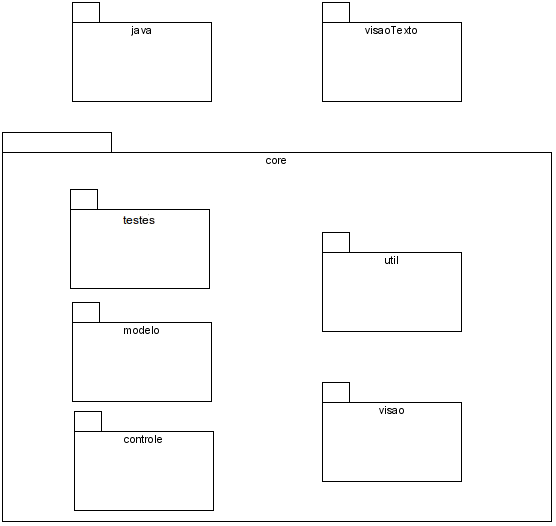
\includegraphics[width=0.5\textwidth]{imagens/Pacotes.png}
  \caption[Diagrama de pacotes do projeto]{Diagrama de pacotes do projeto}
  \label{diagrama-pacotes}
\end{center}
\end{figure}


\begin{description}
  \item[com.mac242.guerradasuniversidades.java] Pacote gerado pelo PlayN, contém
  apenas uma classe, a GuerraDasUniversidadesJava, responsável por realizar a
  ligação entre a implementação agnóstica de plataforma (Pacote \texttt{core}) e
  a implementação Java.
  \item[com.mac242.guerradasuniversidades.core.modelo] Pacote contendo o
  modelo lógico do jogo
  \item[com.mac242.guerradasuniversidades.core.visao] Pacote contendo a
  interface gráfica implementada com o PlayN
  \item[com.mac242.guerradasuniversidades.core.controle] Pacote contendo o
  controle da interface gráfica, também implementada com o PlayN
  \item[com.mac242.guerradasuniversidades.core.testes] Testes unitários do
  modelo.
  \item[com.mac242.guerradasuniversidades.core.util] Classes utilitárias
  não relacionadas ao projeto diretamente.
  \item[com.mac242.guerradasuniversidades.visaoTexto] Pacote contendo uma
  interface em modo texto.
\end{description}


\section{Modelo Lógico}
O funcionamento do jogo é bastante centrado nas capacidades e ações de cada
jogador interagindo entre si, sendo necessário apenas uma gerência dessas
interações. Como consequência, o código apresenta como classes principais as
classes \texttt{GuerraDasUniversidades} e \texttt{Jogador}.

A classe \texttt{GuerraDasUniversidades} é responsável por todos os eventos de
responsabilidade do jogo como um todo, sendo uma \textbf{Fachada}
\cite{gof-design-patterns} para o jogo em si. Suas atribuições incluem: Contagem
do tempo, inicialização dos jogadores e ser o informante de eventos ocorridos no
jogo através do padrão Observador-Observado.

A definição das atribuições de um jogador genérico é definida através da
interface \texttt{TipoJogador}. Na implementação final duas classes implementam
tal interface: \texttt{Jogador} e \texttt{JogadorMaquina} correspondendo a 

A classe \texttt{Jogador} cuida das particularidades de um único jogador, tais
como seus PE, FO, maxFO, maxPE, etc. A única exceção é a gerência das estruturas
compradas ou compráveis, que fica a cargo do \texttt{GerenteEstruturas}. Como
cada estrutura possui sua particularidade e para preservar a extensibilidade
futura a equipe preferiu que cada estrutura tenha seu próprio método de
compra e destruição no \texttt{GerenteEstruturas}.

\texttt{JogadorMaquina} é responsável por implementar a lógica de inteligência
artifical dos jogadores oponentes no jogo, o que é feito no método
\texttt{realizarJogada()}. Além desta atribuição ela deveria reimplementar os
métodos de \texttt{Jogador} que não foram modificados. Para evitar a repetição
de código e evitar os problemas da herança tradicional de código foi realizada
uma \textbf{herança através de composição}, \texttt{JogadorMaquina} delega a uma
instância de \texttt{Jogador} interna as tarefas de controle das informações do
jogador.

Todas as classes que implementam \texttt{TipoJogador} e o 
\texttt{GerenteEstruturas} são internas ao jogo. Por este motivo, elas trabalham
segundo o modelo de programação por contrato \cite{meyer-design-by-contract}.
A API de um jogador, que implementa todos os tratamentos de dados é chamada
\texttt{FachadaJogador} e pode ser obtida por meio do
\texttt{GuerraDasUniversidades}.

Diversos enums foram utilizados ao longo do modelo para
representar diversas informações constantes ao longo do jogo:
\texttt{FocoAdministracao} trata do do enfoque escolhido pelo jogador (Humanas,
Biológicas, etc.). \texttt{NomeUniversidade} inclui o nome das universidades que
o jogo reconhece. Além disso é utilizado como identificador único de um jogador.
\texttt{ResultadoAtaque} representa os diferentes resultados de um ataque, de
Sucesso a falta de FO, falta de uma sala completa etc. \texttt{TipoNotificacao}
representa os diferentes tipos de eventos que acontecem dentro do jogo e que são
informados a observadores externos. \texttt{Estrutura} representa todas as
estruturas e acontecimentos no jogo que podem ser comprados.

Por fim, as classes de status \texttt{StatusJogador} e \texttt{StatusSalaAula}
são objetos simples e descartáveis que representam informações instantâneas de
um jogador ou sala de aula.

%\usepackage{graphics} is needed for \includegraphics
\begin{figure}[htp]
\begin{center}
  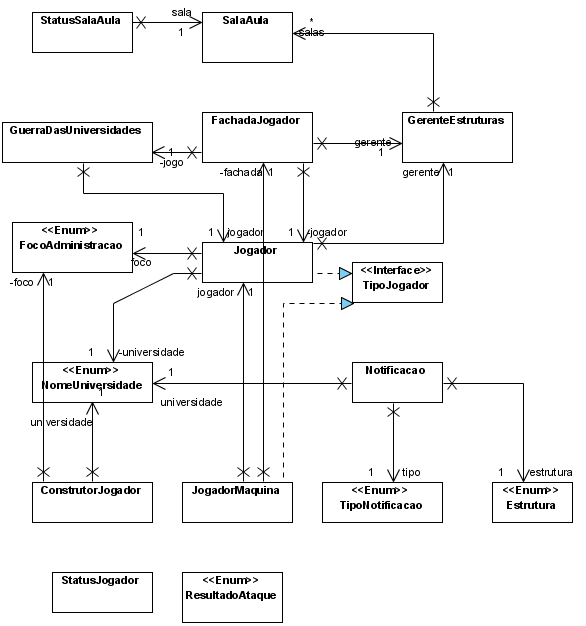
\includegraphics[width=0.9\textwidth]{imagens/ModeloSimples.png}
  \caption[Diagrama de classes simplificado do modelo lógico]{Diagrama de
  classes simplificado do modelo lógico}
  \label{modelo-simples}
\end{center}
\end{figure}

%\usepackage{graphics} is needed for \includegraphics
\begin{figure}[htp]
\begin{center}
  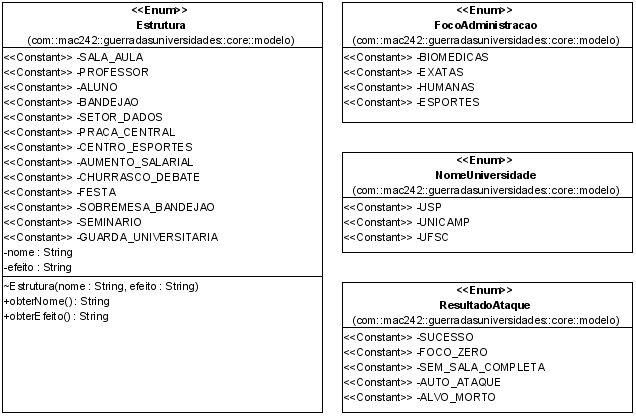
\includegraphics[width=0.8\textwidth]{imagens/Enums.png}
  \caption[Enums do modelo lógico]{Enums do modelo lógico}
  \label{enums}
\end{center}
\end{figure}

%\usepackage{graphics} is needed for \includegraphics
\begin{figure}[htp]
\begin{center}
  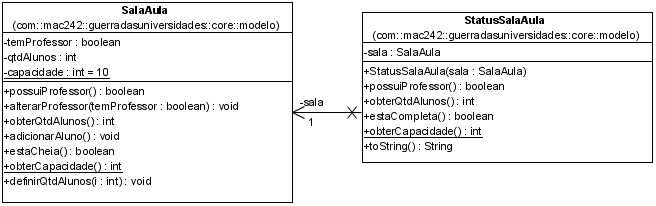
\includegraphics[width=0.8\textwidth]{imagens/SalaAula.png}
  \caption[Classes representantes de uma sala de aula]{Classes
  \label{visao-simples}
  representantes de uma sala de aula}
\end{center}
\end{figure}


%\usepackage{graphics} is needed for \includegraphics
\begin{figure}[htp]
\begin{center}
  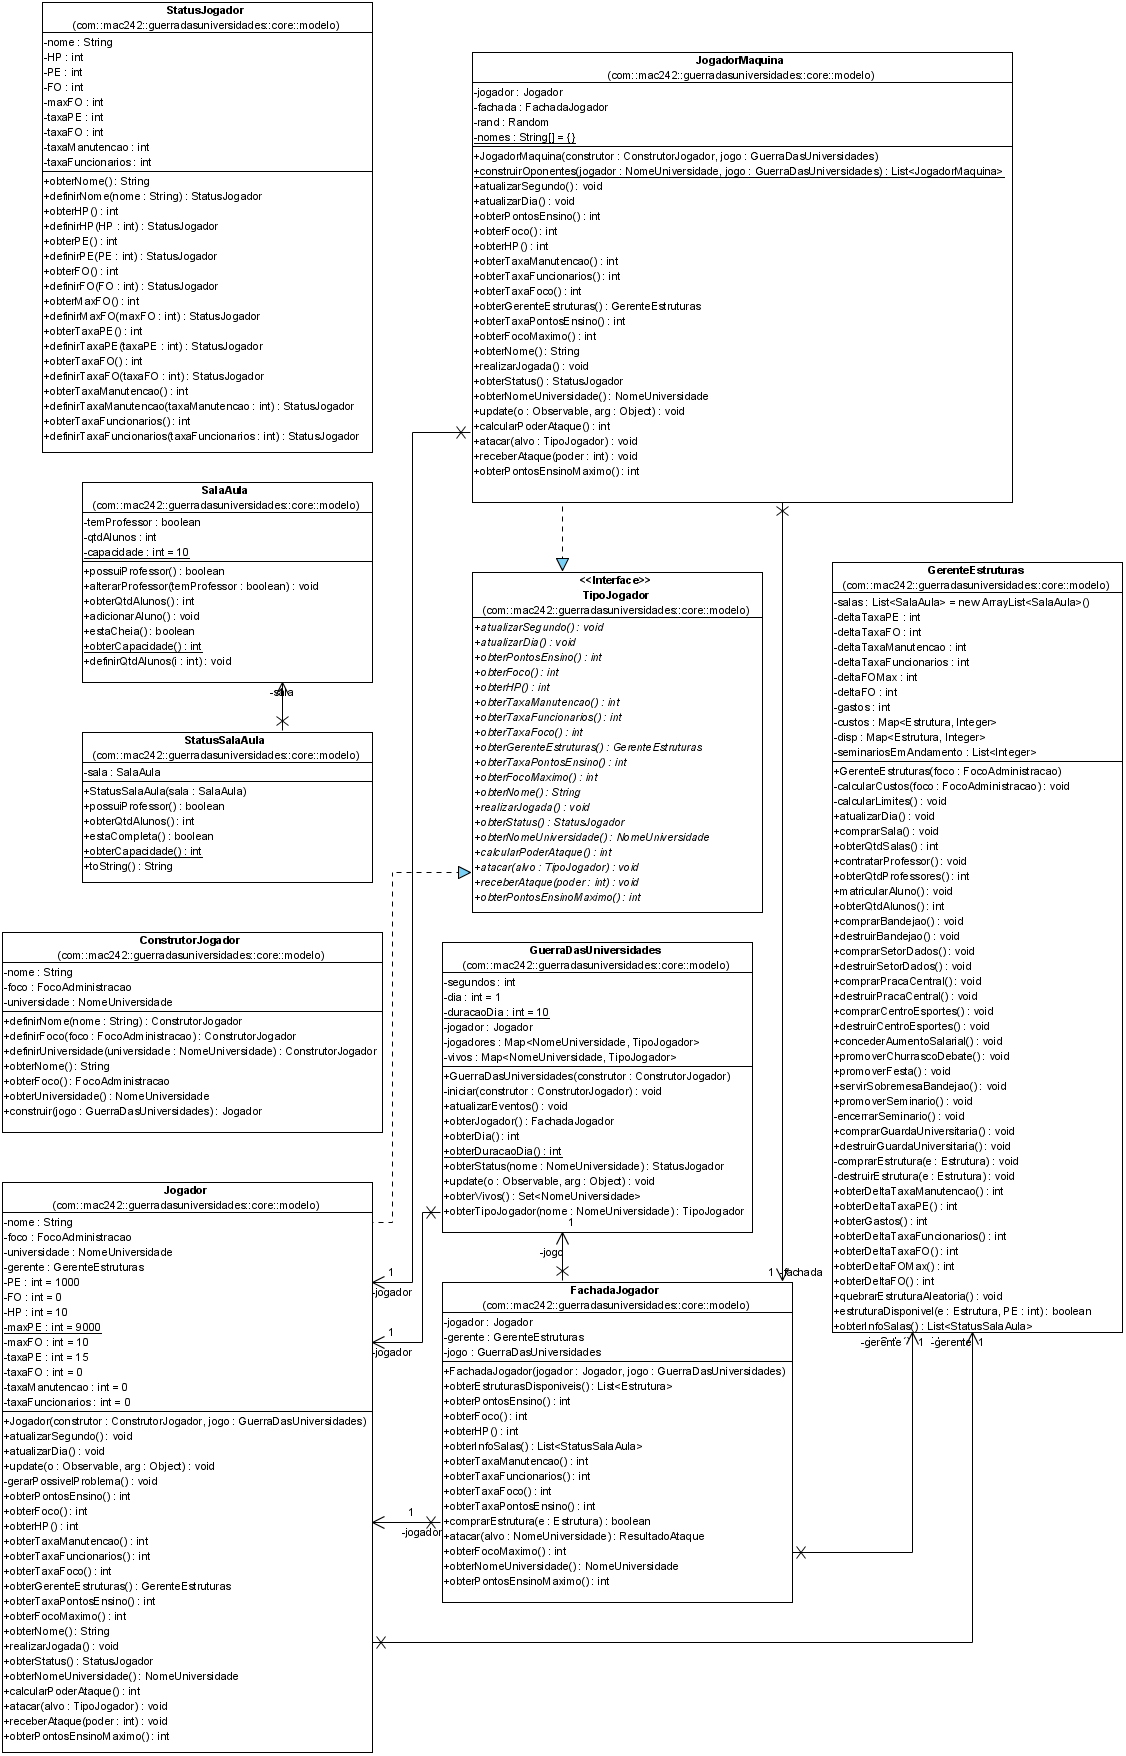
\includegraphics[width=\textwidth]{imagens/ModeloBasico.png}
  \caption[Diagrama de classes do modelo lógico]{Diagrama de
  classes do modelo lógico}
  \label{visao-basica}
\end{center}
\end{figure}

\section{Visão}
A interface gráfica do jogo é composta basicamente de telas, cada uma delas
extende a classe abstrata \texttt{TipoTela}, que contém métodos utilitários
comuns a todas as telas como rotinas de inicialização, atualização e
encerramento de telas e estilos de botões.

O funcionamento de uma tela é baseado em quatro métodos:
\begin{description}
  \item[init()] Inicialização das layers da tela incluindo a base, que deve todas as
outras layers da tela e que será eliminada ao final da exibição dela.
  \item[update(int delta)] Atualização da lógica da tela, chamado regularmente
a cada 10ms.
  \item[paint(int alpha)] Renderização da tela, chamado o máximo
de vezes possível pelo framework.
  \item[shutdown()] Destruição da layer base e quaisquer outras estruturas
  alocadas pela tela.
\end{description}

Cada tela está instanciada apenas uma vez no jogo e essa instância pode ser
acessada a qualquer momento através da classe \texttt{VisaoGuerraUniversidades}.
Esta classe é responsável é a fachada da visão do jogo sendo responsável por
trocar a tela atual e delegar eventos de cliques de mouse aos tratadores
responsáveis. As telas do jogo são: \texttt{Iniciar, Creditos, Ajuda,
KonamiCode, Recordes, Menu, Opcoes, FimJogo}.


%\usepackage{graphics} is needed for \includegraphics
\begin{figure}[htp]
\begin{center}
  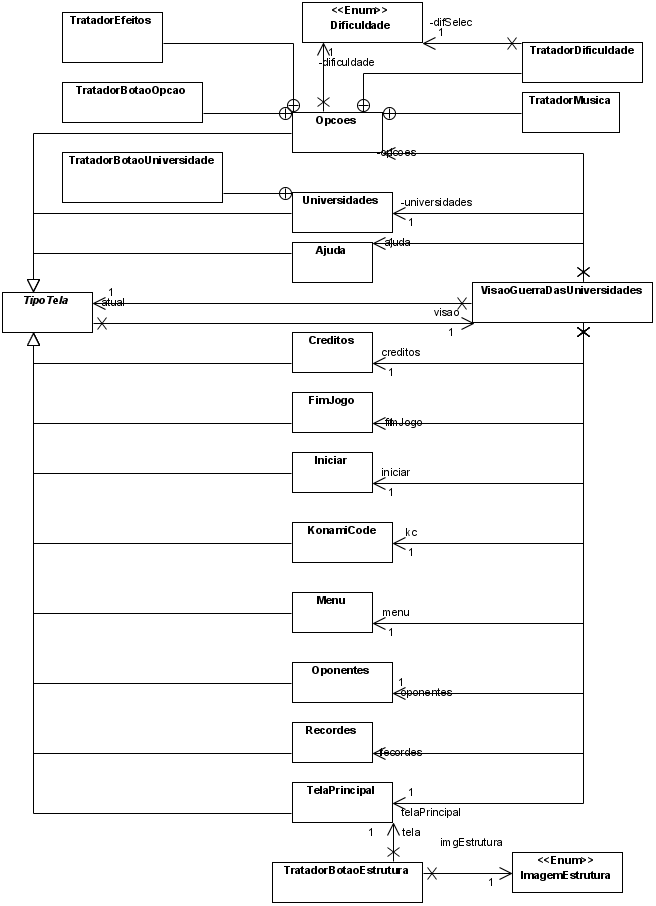
\includegraphics[width=0.8\textwidth]{imagens/VisaoSimples.png}
  \caption[Diagrama de classes simplificado da visão do jogo]{Diagrama de
  classes simplificado da visão do jogo}
  \label{modelo-simples}
\end{center}
\end{figure}

%\usepackage{graphics} is needed for \includegraphics
\begin{figure}[htp]
\begin{center}
  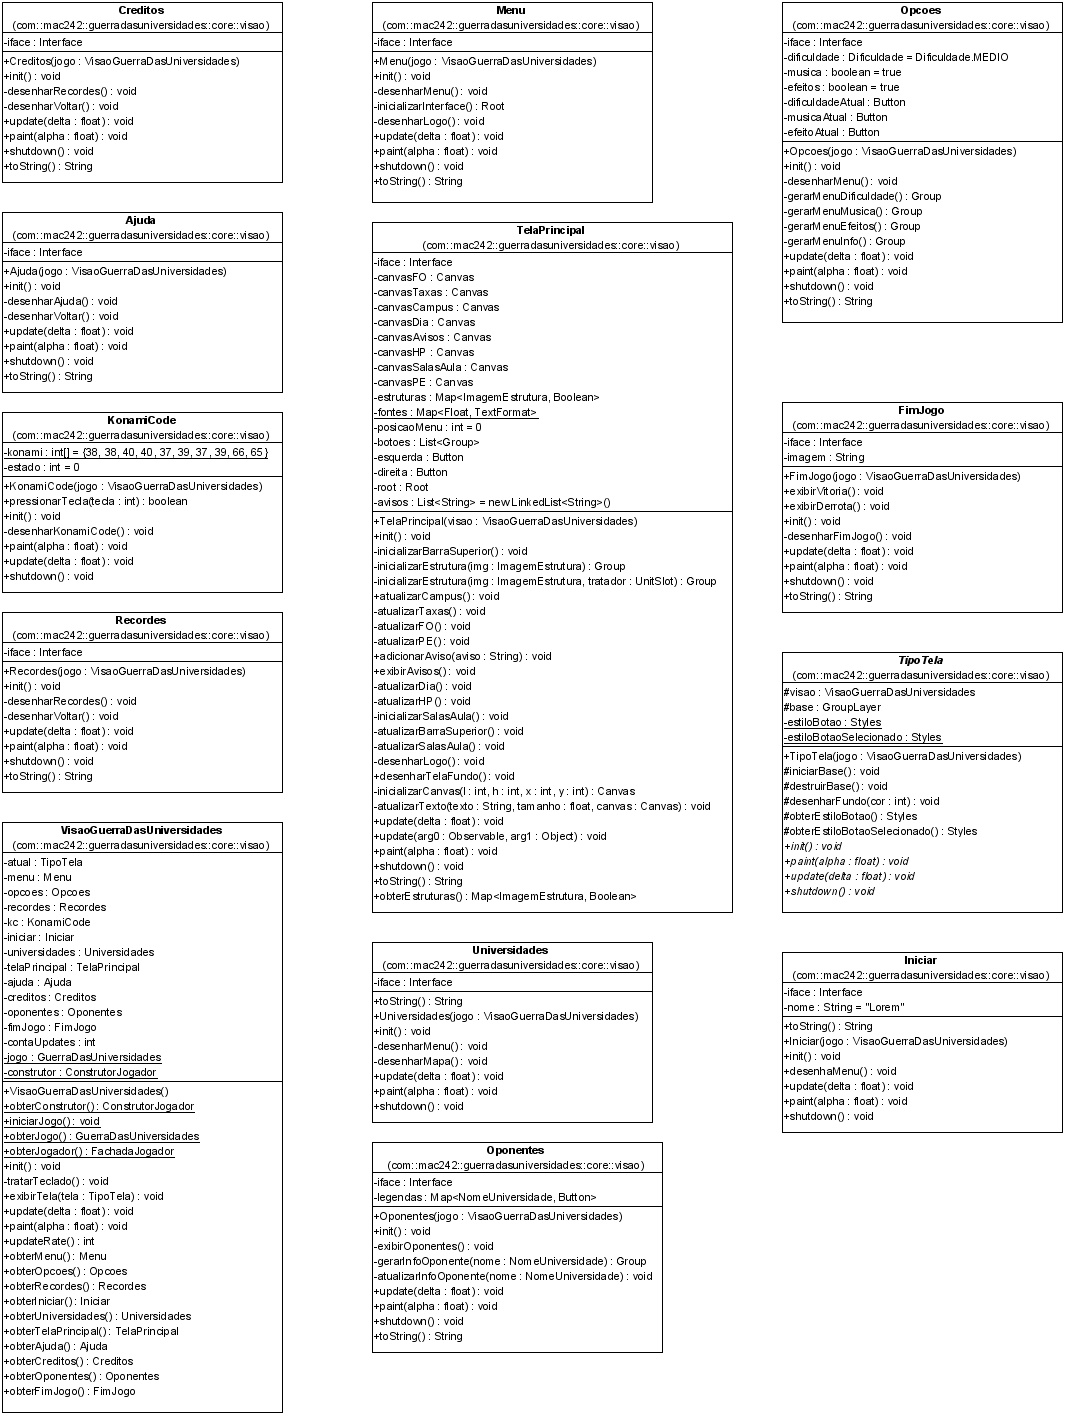
\includegraphics[width=\textwidth]{imagens/TipoTela.png}
  \caption[Diagrama de classes da visão do jogo]{Diagrama de
  classes da visão do jogo}
  \label{modelo-basico}
\end{center}
\end{figure}


\section{Controle}
No pacote com.mac242.guerradasuniversidades.core.controle encontram-se as
classes tratadoras de cliques em diferentes tipos de itens e com diferentes
propósitos. Todos eles realizam a tradução entre intenções do jogador na
interface em ações interpretáveis pelo modelo. Estão implementadas as seguintes
classes: \texttt{TratadorBotaoBlocoEnsino e TratadorBotaoEstrutura} responsáveis
pela invocação de ações de compra de estruturas. \texttt{TratadorTrocarTela}
responsável por invocar a \texttt{VisaoGuerraDasUniversidades} para realizar a
troca de tela. \texttt{TratadorAtacarOponente} responsável por invocar ataques a
oponentes no jogo.

%\usepackage{graphics} is needed for \includegraphics
\begin{figure}[htp]
\begin{center}
  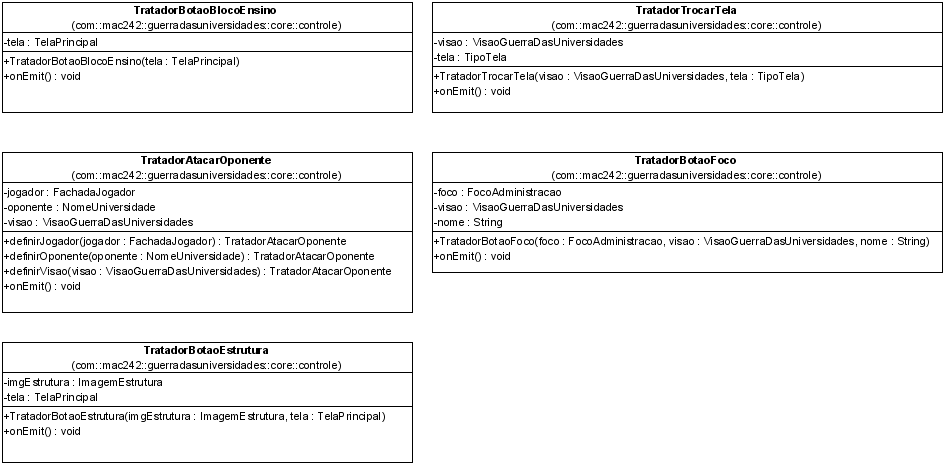
\includegraphics[width=\textwidth]{imagens/Controle.png}
  \caption[Diagrama de classes do controle do jogo]{Diagrama de classes do
  controle do jogo}
  \label{modelo-basico}
\end{center}
\end{figure}

\section{Testes}
Foram implementados testes unitários utilizando a biblioteca JUnit para
garantir o bom funcionamento das classes do modelo. As classes de testes
encontram-se em \texttt{com.mac242.guerradasuniversidades.core.testes}.

\section{Utilitários}
O pacote \texttt{com.mac242.guerradasuniversidades.core.util} contém duas
classes, \texttt{Observer e Observable} que implementam o padrão de projeto
Observador-Observado. Elas são cópias fieis de \texttt{java.util.Observer}
e \texttt{java.util.Observable} obtidas de código licensiado pela GPL pela
antiga Sun Microsystems, atual Oracle. Isso foi feito pois o GWT não fornece
tais classes no subconjunto da API do Java que é traduzível para Javascript.
Isso impossibilitaria o \emph{deploy} para a web no Google AppEngine.


\chapter{Documentação do Código}\label{documentacao-codigo}
Como dito anteriormente, o código fonte foi documentado utilizando a ferramenta
Javadoc, responsável por gerar automaticamente uma documentação das classes,
interfaces, enums, métodos etc. Tal documentação está localizada em Documentacao
no formato HTML. Para lê-la abra o arquivo \texttt{index.html} em algum
navegador web.

\bibliographystyle{abnt-num}
\bibliography{bibliografia}
\end{document}